%!TEX root = RBM.tex

\subsection{Estimating Results}

We estimate the results of the three algorithms using 4 models with 10, 20, 100, 500 hidden units respectively, all 4 models have 784 visible units. The models are trained by the MNIST handwritten digit dataset\cite{lecun1998mnist}.

Note that we only calculate the real value of the partition function in the model with 10 hidden units ($logZ(\theta)=226.11$), due to my poor laptop has broken down several times when calculating the model with 20 hidden units and maltab doesn't even allow to calculate the other two models because they require unimaginable quantity of memories.

\para{AIS}
\begin{figure}[t]
	\centering
	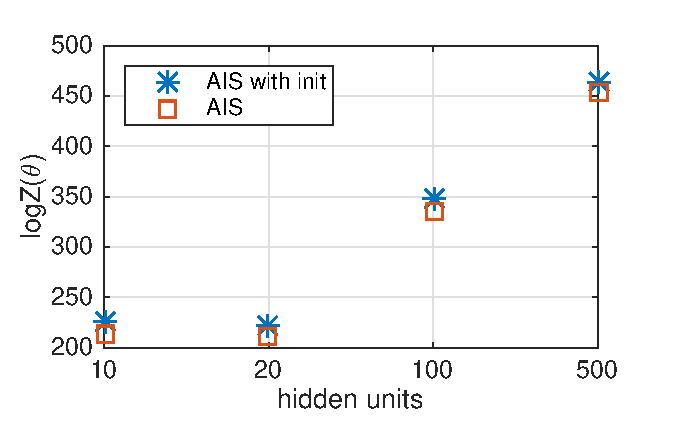
\includegraphics[width=0.48\textwidth]{figure/AIS_results/ais_result.eps}
% \vspace{-0.1in}
	\caption{Comparison of AIS method, with or without an initialization of $\mathbf b$}
\label{fig:aisresult} % FIG1
\end{figure}
By setting number of iteration at 100 times, and $\mathbf \beta$ uniformly sampling from 0 to 1 for 10,000 points.

From Figure~\ref{fig:aisresult}, we can see that the estimation results will differ a lot if we use an initialization method to initialize the visible bias $\mathbf b$, as mentioned in the previous subsection. In a model with 10 hidden units. We see AIS with init almost obtain the real value (226.11) without error.

\para{RTS}



\para{TAP}
\begin{figure}[t]
\begin{minipage}[t]{1\linewidth}
	\centering
  	\subfigure{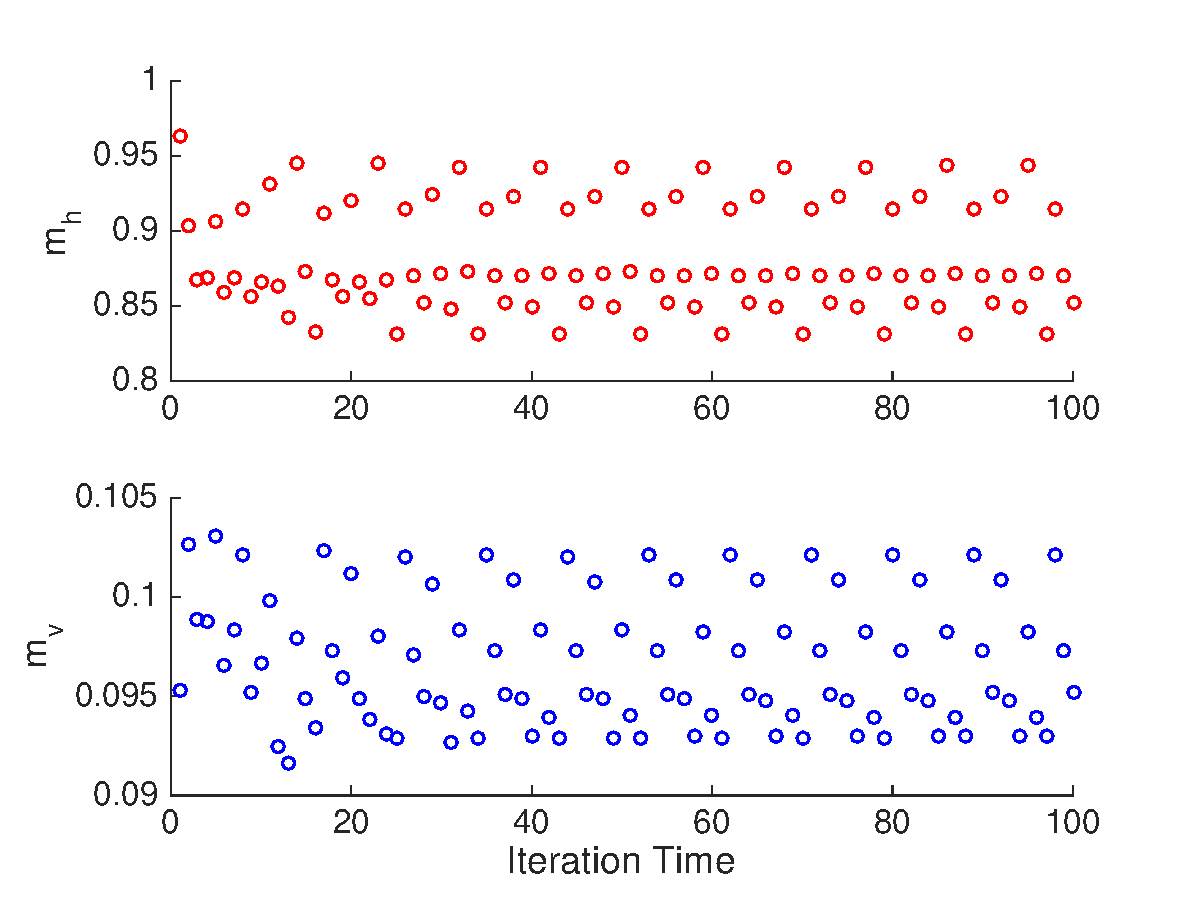
\includegraphics[width=0.48\textwidth]{figure/TAP_results/mvmh_10.eps}}
	\subfigure{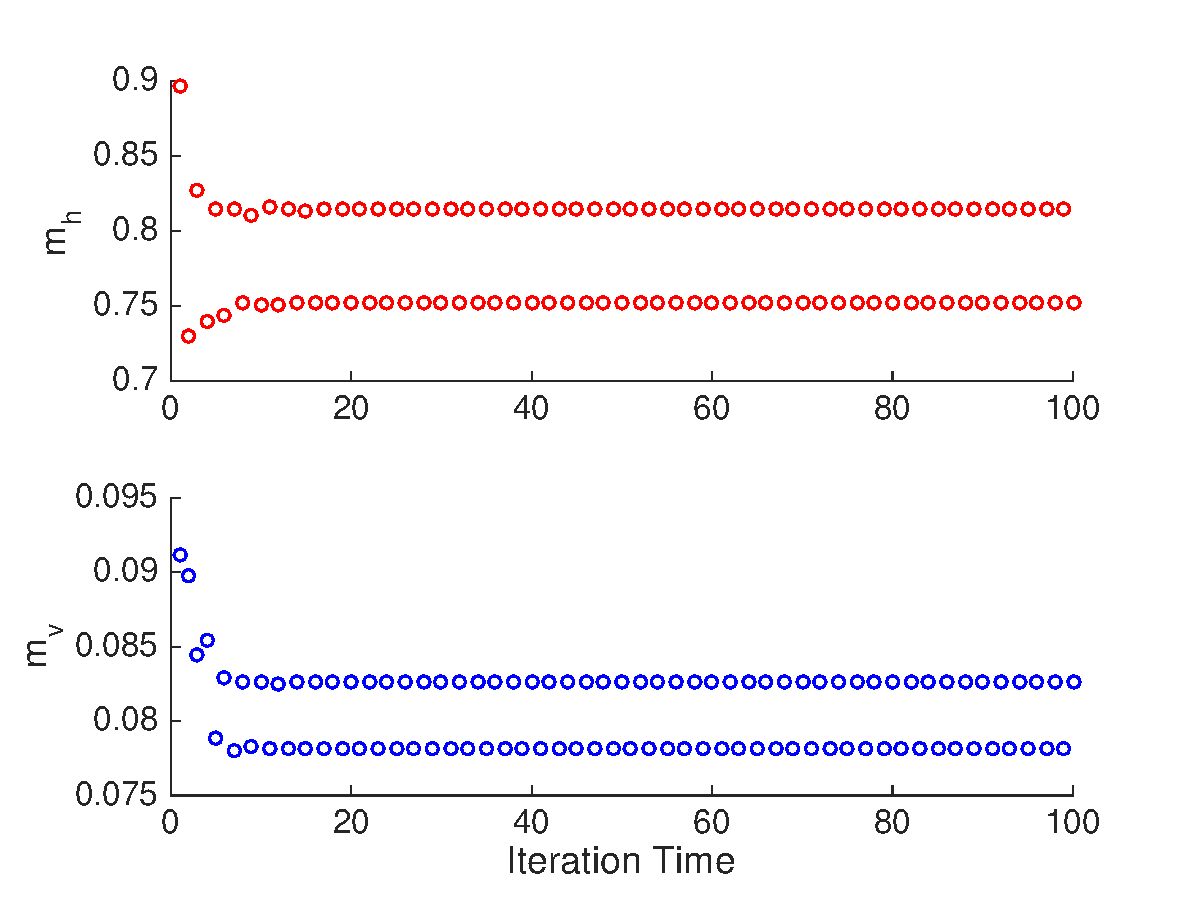
\includegraphics[width=0.48\textwidth]{figure/TAP_results/mvmh_20.eps}}
	\subfigure{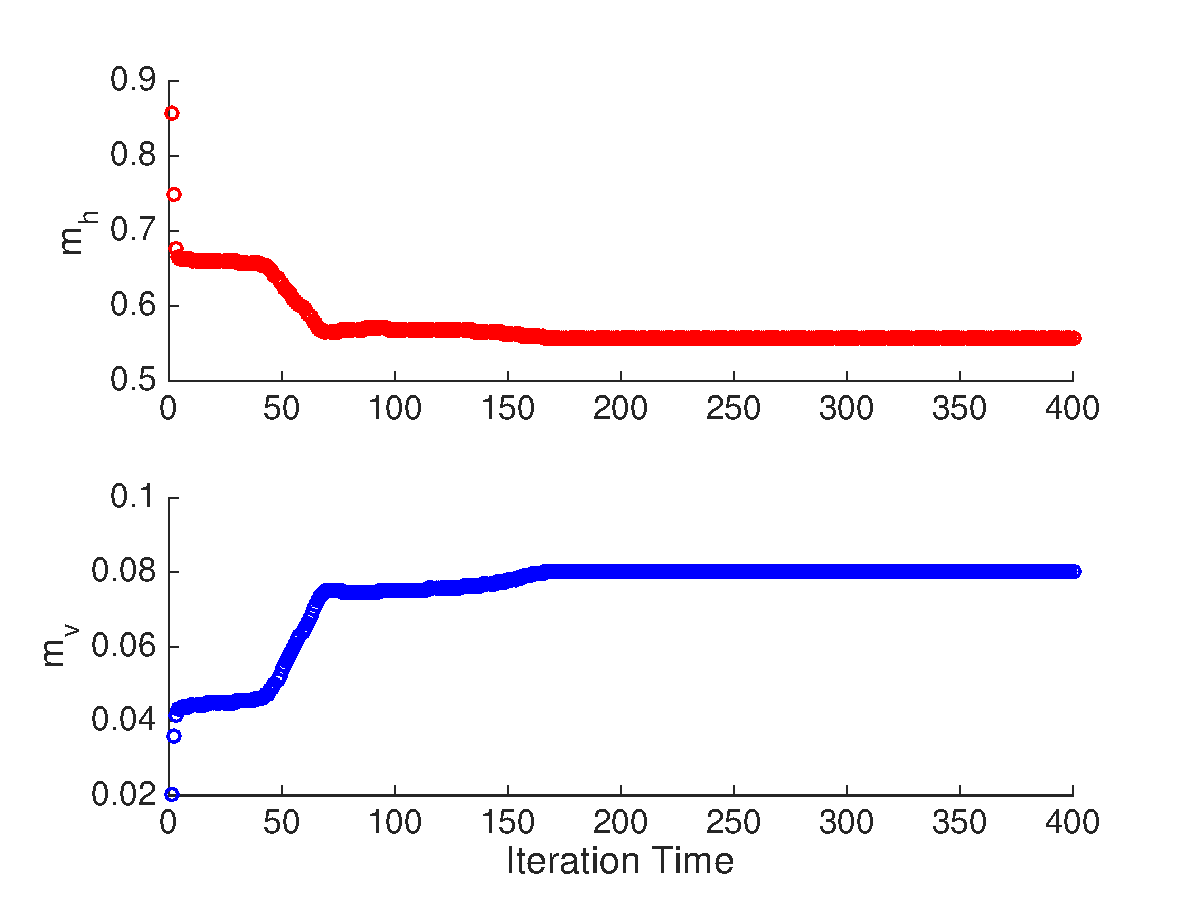
\includegraphics[width=0.48\textwidth]{figure/TAP_results/mvmh_100.eps}}
	\subfigure{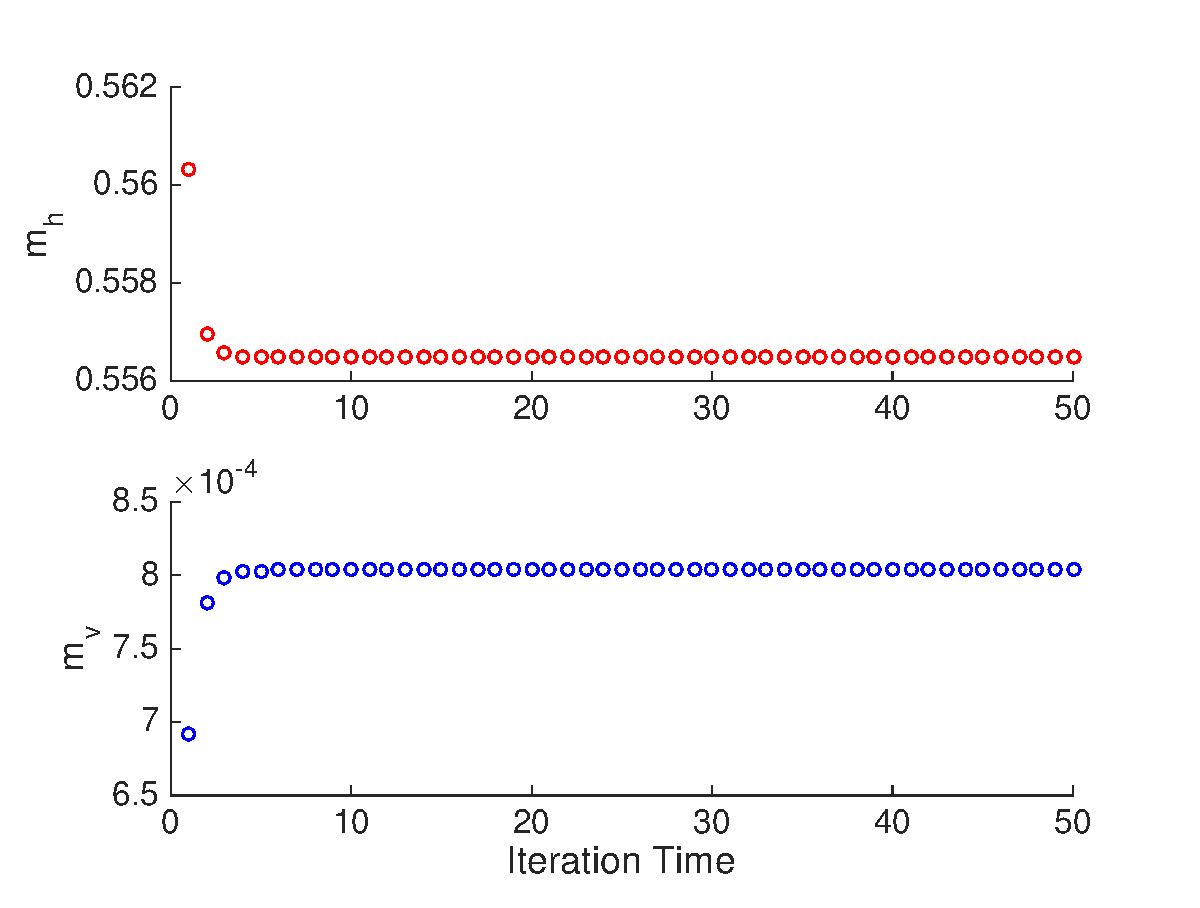
\includegraphics[width=0.48\textwidth]{figure/TAP_results/mvmh_500.eps}}
% \vspace{-0.1in}
\caption{$m_{h}$, $m_{v}$ convergence condition using TAP method. From left to right, up to down, the figure indicates an RBM model with 10, 20, 100, 500 hidden units. The convergence time is approximately 40, 20, 175, 5. By such few iteration time, all results can be obtained in less than 1 second.}
\label{fig:TAPmhmviter} % FIG1
\end{minipage}
\vspace{-0.05in}
\end{figure}
When running a TAP, we see we can get converged $m_{v}$ \& $m_{h}$ in very few iteration time (Figure~\ref{fig:TAPmhmviter}, convergence time is approximately 40, 20, 175, 5 for the model with 10, 20, 100, 500 hidden units respectively). Given this observation, the computing time of TAP is negligeable (we obtain all results in less than a second). 

However we do notice that the converged results are sometimes not consistent but periodic. (eg. Figure~\ref{fig:TAPmhmviter}, when there are 10, 20 hidden units), this is not a good news because even if we have more resources to compute the iterations, we would not have a better result.

And disappointingly, compared to the result of other algorithms (Figure~\ref{}), TAP usually have a lower estimation value, which is not preferable.







If we don't consider time \& resources, we can get good results for all three methods(Figure x).
